\chapter{Review of Institutional and Open Learning Spaces \label{cha:systudy}}

This review focuses on technical aspects of lifelong learning support.
Therefore, the following sections examine characteristics of the learning spaces
employed in universities and describe the issues related to the use of these
spaces in a universities environment. A review of \ep~systems is also
provided in these sections.

This review focuses on technical aspects of lifelong learning support.
Therefore, the following sections examine characteristics of the learning spaces
employed in universities and describe the issues related to the use of these
spaces in a universities environment. A review of \ep~systems is also
provided in these sections.

This review focuses on technical aspects of lifelong learning support.
Therefore, the following sections examine characteristics of the learning spaces
employed in universities and describe the issues related to the use of these
spaces in a universities environment. A review of \ep~systems is also
provided in these sections.

\section{Learning Management Systems}
Higher education institutions have fully embraced computer systems to support
teaching and learning. According to a survey conducted by the OECD Centre for
Educational Research and Innovation encompassing universities in 13 countries
89\% of responding institutions were using university-wide LMS. Further
indications of uptake can be seen when visiting institutional websites, looking
at user statistics provided by system suppliers (for example,
\url{http://moodle.org/sites/} or
\url{http://sakaiproject.org/community-home}) or by following discussions in
the academic literature \citep{Browne2006,Collis2004}.

The systems are referred to as Virtual Learning Environments, Course Management
Systems or Learning Management Systems (LMS), the term used in this thesis. A
number of online information and communication tools are usually integrated in
such an environment into a single virtual location \citep{Morgan-Klein2007}
providing users with an access to teaching and learning materials, such as
lecture slides or exercises. A virtual space of LMS is shared by staff and
students of a particular course. This space forms a platform for course
discussions and facilitate assessment, both via online testing and for
submission and return of assignments.

The use of LMS in higher education is characterised by a strong institutional
focus \citep{Siemens2004}. Access to the LMS dependens on current enrolment
with the institution and is organised around course structures. This means
students have access to only the courses they are enrolled in and only for the
duration of these courses. The learning spaces for the different courses a
student is enrolled in are separate. LMS is based on a hierarchy of user access
rights. The lecturer in charge determines the toolset for their course and sets
the parameters that define the involvement of the students. The lecturer has
access to all information stored for their course in the LMS, leaving no or only
very limited private space for the student. The content and use of the LMS is
focused fully on the course requirements. As a course-focused virtual learning
space, LMS make a huge contribution to the delivery of both face-to-face and
distance courses in today's universities.

\section{Web 2.0 and Social Virtual Spaces}
Outside the higher education sector, in the open Internet domain, the Web 2.0
social networking tools have been firmly established. Tools are available for
the sharing of images, photos and video clips. Individuals can communicate with
others in synchronous and asynchronous forms, and in access-protected as well as
open formats. Individuals can consume information on the widest possible range
of topics and can as well contribute. Web 2.0 is characterised by open access,
availability to anyone who has an Internet connection, and with the level and
kind of participation determined solely by the individual. With freedom comes
responsibility, and the responsibilities for taking up opportunities as well as
for 'safe' conduct in the Web 2.0 space lie with the individual.


\begin{figure}[htb]
\centering
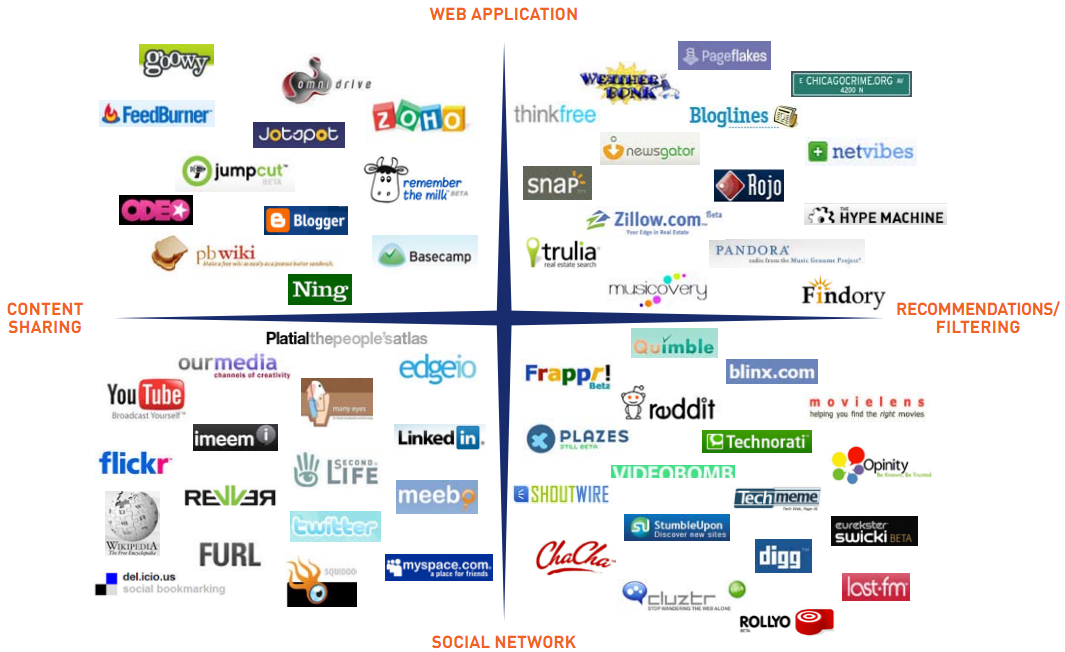
\includegraphics[width=1\textwidth]{CH4-F0-WEB20}
\caption[Web 2.0 Landscape]{Web 2.0 Landscape \citep{Dawson2007}}
%http://www.rossdawsonblog.com/Web2_Framework.pdf
\label{fig:web20l}
\end{figure}

Web 2.0 plays an important role in today's society and is used for social and
commercial purposes. Examples from a variety of areas show the popularity and
impact of Web 2.0: Virtual sports leagues attract millions of participants
\citep{Holahan2006}; politicians use blogs and podcasts in fighting for
voters \citep{Capell2006}; communication with customers are used to increase
revenue (Havenstein, 2007); communication pathways in research communities are
changing \citep{Ashling2007}; video-blogging facilitates new ways of sharing
(Library Technology Reports, 2007); the music industry is being transformed
\citep{Holahan2007}; genealogy research has become accessible to the public
\citep{MacMillan2007}.

Certainly not all uses of Web 2.0 are linked to learning, especially when
thinking of the higher education context. But, in light of the lifelong learning
skills expected from today’s higher education graduates, the potential of Web
2.0 for supporting learning becomes obvious. This potential is confirmed by
research studies that investigate the links between the two areas: Churchill
\citeyear{Churchill2009} examines the use of blogs in support of learning; Wheeler,
Yeomans and Wheeler \citeyear{Wheeler2008} look at student-generated content using
wikis; Boulos and Wheeler \citeyear{Boulos2007} investigate Web 2.0 tools for
social communication in a learning context. Yet, when designing education that
integrates Web 2.0 technologies the skill levels of students have to be
considered. While it is widely assumed that today’s student generation is
Internet savvy, it has to be acknowledged that quite a number of students have
limited Web 2.0 skills. They are either not familiar with the technologies, or
have only basic level skills (Kennedy et al., 2008).

\section{Gap Between Learning Environments}
Students in higher education have access to both environments, the
institutionally focused LMS and the individually focused Web 2.0. On large,
these two virtual worlds remain separate, both in the students’ and the
institutions’ minds, with a distinction being made between ‘serious learning’
and ‘play’.  Many students cannot transfer their technology skills employed in a
social Web 2.0 context into academic learning, which is both a motivational and
a skill transfer issue (Katz, 2005). The information technology sections of
institutions draw a clear line between institutionally provided, controlled and
supported LMS services and the ‘wild west’ of the Web. While they cannot
effectively restrict access to Web 2.0 tools they can deny institutional support
and responsibility for quality of service. Educational researchers and
individual academics have identified the potential of social networking tools
for teaching and learning. This has led to the incorporation of open access Web
2.0 tools into some courses in higher education, as we have illustrated earlier.

In response to the popularity of Web 2.0 tools and their potential for learning,
LMS system providers have started to integrate social networking functionality
into their systems. Discussion forums, blogs and wikis have been added to the
toolsets of LMS. Yet, the important Web 2.0 characteristic of open access has
been removed as these tools have been bound into the institutional LMS
framework. Access is linked to course enrolment and under institutional control.
Student generated content is accessible to the lecturers in charge and tool use
is directed by relevance to the respective course. This still leaves us with
value for teaching and learning, yet confines learning to the boundaries of
course content and purpose.

\section{ePortfolio}
For a long time physical portfolios have been used by artists as presentation
tools to collect, organize and showcase their artwork. The aim was to convince
potential customers of their competence. Two decades ago portfolios were adopted
by educators to assess the quality of teaching \citep{VanTartwijkJ.2004}. Since
then portfolios have been used for many different purposes which defined such
types of portfolios as showcase, development and assessment.

Electronic portfolios or ePortfolios are a digital representation of physical
portfolios. The EDUCAUSE National Learning Infrastructure Initiative
(NLII)\footnote{\url{http://www.educause.edu}} (cited by
\citealp{IMSGlobalLearningConsortium2005}) defines ePortfolio as:

\longquote{ePortfolio is a collection of authentic and diverse evidence, drawn
from a larger archive, that represents what a person or organization has learned over time,
on which the person or organization has reflected, designed for presentation to
one or more audiences for a particular rhetorical purpose.}

\subsection{Characteristics of Portfolios and ePortfolio Systems}
The term portfolio is used in many different ways. One important distinction can
be made along the lines of purpose of a portfolio, namely for development,
showcase, assessment or competences. Development portfolios or repositories
support the learning and development of a learner. They contain material and
artefacts related to learning, reflections and feedback. It is important that
the material stored in these repositories is private to the learner. It is up to
the learner to decide when and what to share with whom. The learner needs to
reflect on the material collected and on his/her development in relationship to
criteria or skills. The giving and receiving of feedback are important aspects
of the learning processes around development portfolios. Showcase or
presentation portfolios allow the learner to present their work and development
to others. These presentations contain reflection and supporting evidence. They
are composed for a specific purpose and audience, e.g. an assessment committee
or a potential employer.

Portfolios are often linked to assessment. Type of portfolio and type of
assessment have to be carefully adjusted to each other. Assessment portfolios
demonstrate learner's competencies and skills in well-defined areas. They can be
used for both formative and summative assessment. For formative assessment the
learner documents work and reflects on it, the assessor provides feedback that
assists the learner in future development. Summative assessment requires
predefined criteria of what is to be assessed allowing the learner organize work
examples according to these criteria. In the design of the assessment approach
one has to be very careful to specify clearly what is to be assessed: subject
specific work, reflections, \LLLs skills, or presentation.

Development portfolios or repositories support and keep track of the learning
and development of a learner over a period of time. They contain material and
artefacts related to work-in-progress, reflections and feedback. Reflection as
well as the giving and receiving of feedback are important aspects of
development portfolio.

Showcase portfolios tend to display examples of learner's best work. These
presentations contain reflection and supporting evidence. They are composed for
a specific purpose and audience, e.g. a review committee, potential employer or
sponsor.

Portfolios for competences combine elements of both development and showcase
portfolios and are, to a certain degree, linked to assessment. In professional
areas, like health services, teacher education or engineering, the accreditation
of graduates and the continuing accreditation of professionals are often linked
to the demonstration of competencies. Portfolios have proven to be excellent
tools for this process. The candidate collects evidence, reflects on their
practice and might invite feedback, all processes covered by portfolio
approaches. The accreditation occurs based on the information provided in the
portfolio.

Despite these variations, there are several key processes included in most if
not all portfolio work, as is displayed in \ref{fig:ep}.
 
\begin{figure}[htb]
\centering
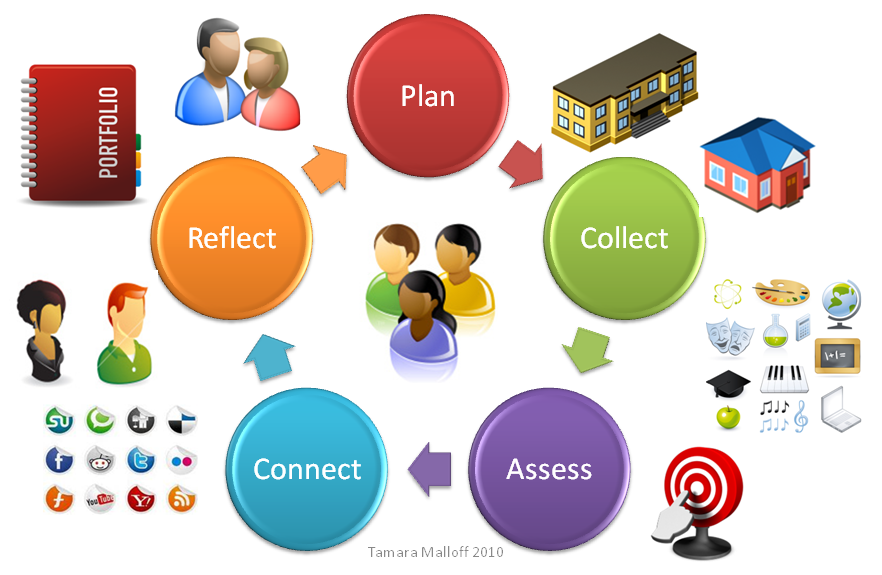
\includegraphics[width=0.8\textwidth]{CH4-F1-EP}
\caption[ePortfolio key processes]{ePortfolio key processes \citep{Malloff2010}}
%http://www.flickr.com/photos/kootenayleadership
\label{fig:ep}
\end{figure}

Similarly, Cambridge \citeyearpar{Cambridge2010} emphasized the importance of
the following activities in portfolio process:

\begin{itemize}
  \item Capture -- collecting/gathering information and evidence from various
  sources;
  \item Management -- aggregating captured evidence, sorting, indexing, ensuring
  accessibility over time;
  \item Reflection -- making sense of evidence, understanding own experience and
  achievements;
  \item Composition -- linking up the components together and making them
  available to others;
  \item Analysis -- understanding if additional evidence is needed, reflecting
  on feedback, keeping up dialog with others.
\end{itemize}

While portfolio work can be conducted without the help of electronic systems,
such systems assist with many tasks around document collection, recording of
information, sorting through data and communicating with others. Many systems,
from general Web tools to specialised applications, can be used to support
portfolio work. A comprehensive overview can be found at Helen Barrett's
ePortfolio site \citep{Barrett2008}. In our chapter we want to concentrate
on systems specialised for portfolio work.

\ep~systems focus on the individual. They provide the individual with a
space for storing documents of any electronic format. In this space the user
creates a repository of artefacts related to all aspects of their learning and
professional development. There are tools for reflection, commonly in form of
blogs. In contrast to open Web 2.0 systems, access to both files and reflections
is by default set to the individual. There is no hierarchy between users in
which one higher-level user could see the work of a lower-level user. The
individual can select to share their work with others and has full control over
whom to share with, for which period of time. ePortfolio systems provide easy to
use tools for constructing presentations that combine artefacts and reflections
and that can voluntarily be shared with others. The systems allow each
individual to form groups and identify partners for exchange. To a varying
degree the ePortfolio systems incorporate guidance towards reflection and
self-directed learning. \ep~systems provide a set of features that in
combination are well suited to support lifelong learning. Each of the features
looked at separately can be found in other computer systems or Web 2.0, but
their combination within one system makes ePortfolios systems so valuable.

\subsection{ePortfolio Systems Overview}
The following sections explore the features and functionality of various
\ep~systems. Four proprietary (PebblePad, BlackBoard \ep, Desire2Learn, eFolio)
and two open-source (Mahara, ELGG) systems are reviewed and analysed. Where
possible, proprietary systems were reviewed by accessing demonstration web
sites. In case demonstration web sites were not available, the systems were
reviewed by analysing user or administrator documentation and external reviews.
These specific systems were chosen for their level of success in learning
communities and current development status. 

It is important to note here that this section is not aiming to find the best
system, but to rather to evaluate \ep~systems that are currently available and
successful. Examining strengths and weaknesses of these systems can provide a
better foundation for understanding and development of an \ep~aided environment
that could support \LLLsn.

%WHERE POSSIBLE NEED SCREENSHOTS OF EPORTFOLIO SYSTEMS%

\subsubsection{PebblePad}

PebblePad\footnote{\url{http://www.pebblepad.co.uk}} is a proprietary web-based
Personal Learning Environment or \ep~system. The system is primarily
used in the UK Higher Education sector and has been involved in a number of JISC
funded ePortfolio research projects including
ePistle\footnote{\url{http://www.jisc.ac.uk/whatwedo/programmes/edistributed/epistle}}
and File-Pass\footnote{\url{http://www.jisc.ac.uk/whatwedo/programmes/edistributed/filepass}}.

\begin{figure}[htb]
\centering
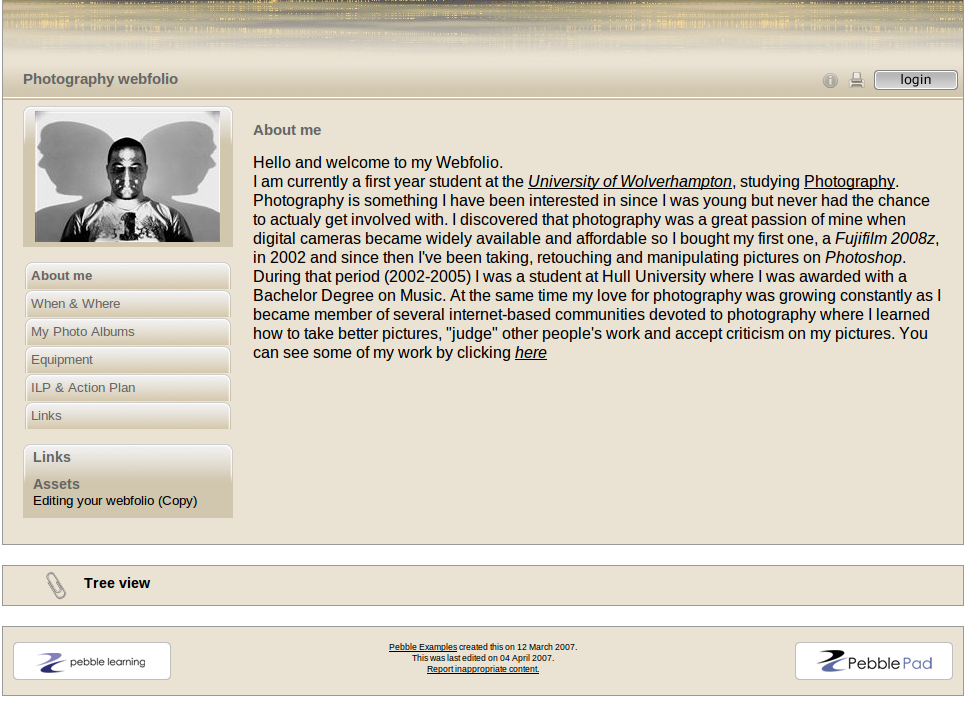
\includegraphics[width=0.8\textwidth]{CH4-F3-PebblePad}
\caption[PebblePad ePortfolio system example]{PebblePad ePortfolio system example
\citep{PebbleLearningLtd}}
\label{fig:ppep}
\end{figure}

The system provides six structured input forms to record skills, experiences and
reflections. Additionally, users can define any file type and add it to their
asset store. PebblePad provides an opportunity to aggregate artefacts into
WebFolios to share with others, inside or outside of an institution, for certain
periods of time through user-defined permissions. This system also supports
collaboration allowing collectively creating items for joint projects.

PebblePad has a newly developed Moodle block that allows \ep~users to have
single sing-on with LMS and also export items from Moodle to their ePortfolio.
The system supports export and import of personal portfolios through LEAP2A
export format.
 
\subsubsection{Mahara}
Mahara\footnote{\url{http://mahara.org}} is an \ep~system started in 2006 and
funded by New Zealand Tertiary Education Commission. The system is a standalone
web application and does not require any kind of LMS or another system
installed. Its big advantage over other \ep~systems is in its modular and
extensible architecture that resembles the architecture of Moodle LMS. This can
be explained by the fact that developer community of Mahara is deeply involved
in the Moodle community. The system is claimed to be highly 'pluggable' which
allows adding various Web 2.0 web services and establish interoperability with
other systems \citep{MaharaGovernanceGroup2011}.

\begin{figure}[htb]
\centering
\setlength\fboxsep{0pt}
\setlength\fboxrule{0.5pt}
\fbox{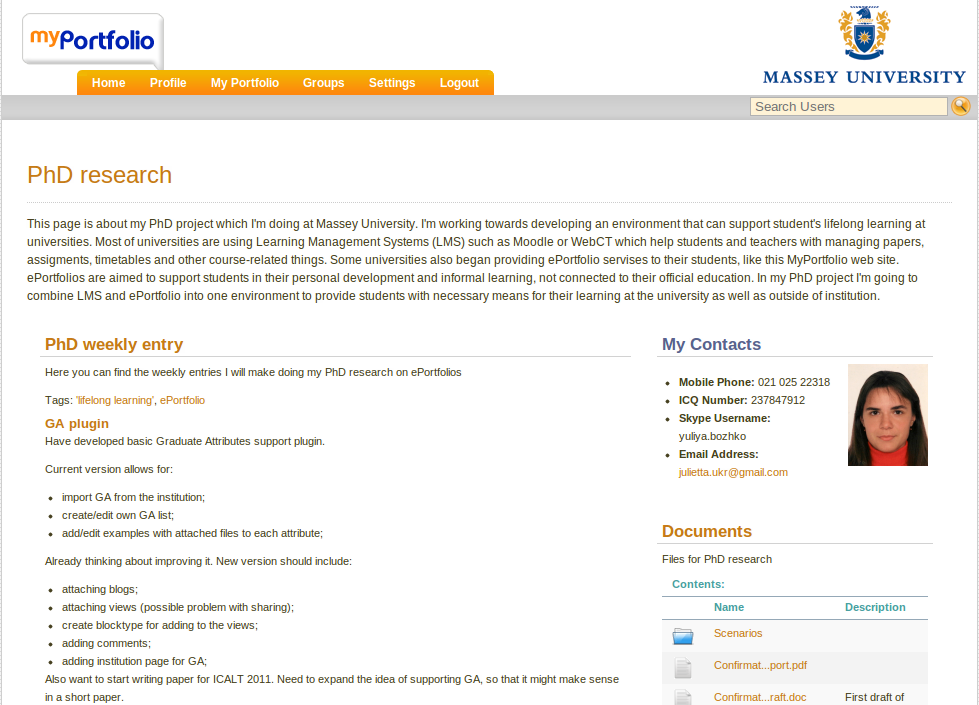
\includegraphics[width=0.8\textwidth]{CH4-F4-Mahara}}
\caption{Mahara ePortfolio 1.3 example}
\label{fig:maharaep}
\end{figure}

Mahara functionality includes a number of standard \ep~features like file
repository, reflection tools in form of blogs, presentation and sharing tools as
well as elements of social networking like friends lists, forums, message board
and e-mail. Mahara has internal r\'{e}sum\'{e} builder which allows users to
create their digital CV with various information options. Sharing is done
through pages which are called 'views'. Users can create single views or
collections of views and fill them with artefacts from their \ep~repository.
Views can be created from scratch as well as from a template developed by
another user.

As it became popular in ePortfolio systems throughout the recent years
\citep{Waters2009}, Mahara comes with a user-to-user permissions control. Users
can set up three levels of access to parts of their ePortfolios (private,
individual and public) which defines what items and information others can see.
Currently the Mahara system does allow sharing views with others or making them
public, but giving feedback is restricted to registered users.

Mahara supports a complete LEAP2A interoperability which allows to import
portfolio to Mahara and export it to another \ep~system, provided that this
interoperability standard is implemented at the other side. In addition, export
can be done in form of static HTML pages.

Latest version of Mahara supports a single sign-on with Moodle, which means that
users can log on to both systems using only one account. Unofficial plugins
developed by community allow for submitting views as assignments to Moodle.
However, this functionality is not included in official release. The roadmap of
Moodle 2.0 included a repository plugin for Mahara that would allow direct
export of artefacts from LMS to \ep. Meanwhile, Moodle 2.1.1 release still does
not support this functionality.

\subsubsection{ELGG}
ELGG\footnote{\url{http://elgg.org}} is an open source social networking and
social publishing platform started in 2004 and released under the GNU Public
License v2. It was originally aimed at higher education, but is currently used
in many contexts from business to sport. Developers of ELGG call it a 'social
engine to empower social environment'.

\begin{figure}[htb]
\centering
\setlength\fboxsep{0pt}
\setlength\fboxrule{0.5pt}
\fbox{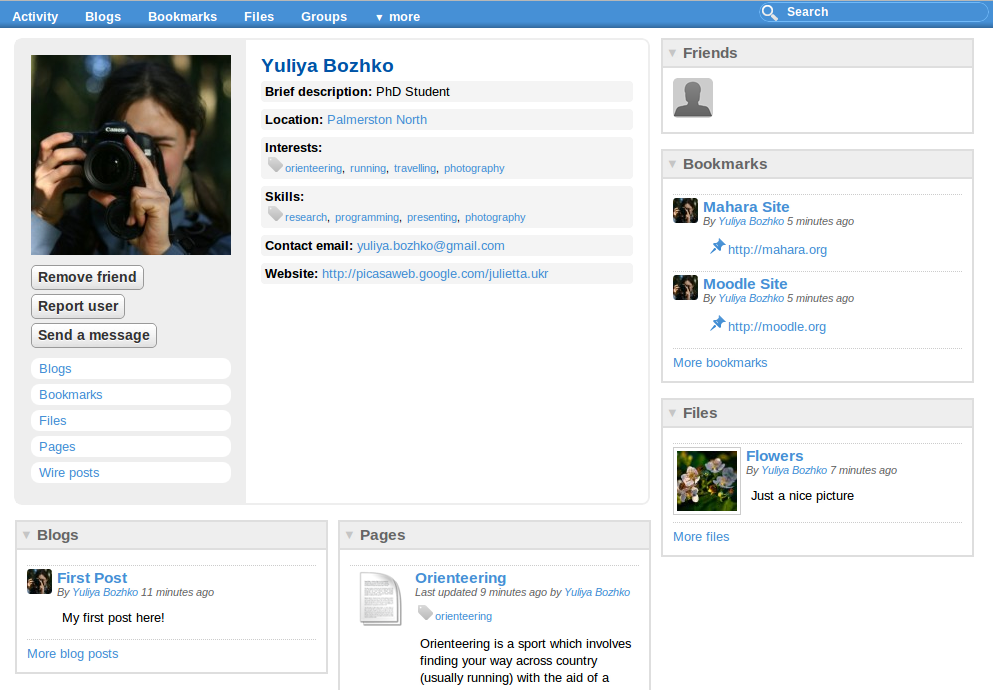
\includegraphics[width=0.8\textwidth]{CH4-F5-ELGG}}
\caption{ELGG 1.8 example}
\label{fig:elgg}
\end{figure}

ELGG comes with built-in features as well as optional plugins. Features
available in the platform include user management and administration, social
networking components, blogging, message board, file repository, private
messaging, pages, and bookmarks. Most the end user functionality comes from
plugins which can be loaded into system. ELGG has an extensive community support
which contributes a large number of its plugins, although in general most of
these plugins are aimed to support social networking.

\subsubsection{BlackBoard ePortfolio}
After merging in February 2006, two popular LMS providers
BlackBoard\footnote{\url{http://www.blackboard.com/}} and WebCT developed an
\ep~toolkit the most recent release of which is currently a part of BlackBoard
Learn 9.1. This \ep~system is designed as an add-on to the LMS environment and
can not be used as a stand-alone product. On one hand, it means that all users
must have BlackBoard LMS account to be able to access \ep. On the other hand, it
gives some advantages which other \ep~systems might lack, such as single sign-on
with LMS, direct import of graded materials from Blackboard courses and links to
course goals and objectives.

BlackBoard \ep~is available in Basic and Personal Portfolio versions. Basic
Portfolio has an \ep~set-up wizard for learners who need guidance. However, it
is largely dependent on functionality available in LMS. Without activation of
various features, the repository might be restricted to text and hyperlinks
only. Personal Portfolio provides more flexibility and functionality, therefore,
it will be reviewed further as BlackBoard \ep.

\begin{figure}[htb]
\centering 
\setlength\fboxsep{0pt}
\setlength\fboxrule{0.5pt}
\fbox{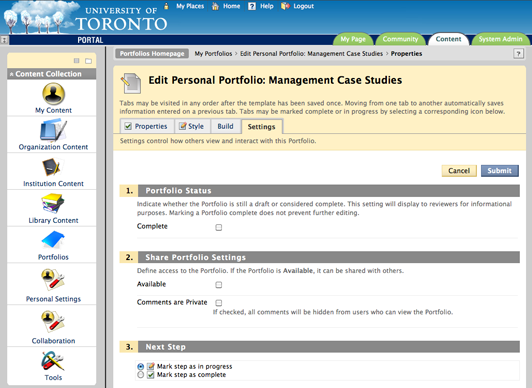
\includegraphics[width=0.8\textwidth]{CH4-F6-BB}}
\caption[BlackBoard ePortfolio example]{BlackBoard ePortfolio example
\citep{UniversityofTorontoScarborough2010}}
\label{fig:bbep}
\end{figure}

In the system, ePortfolio owners have control over the content, access, layout
and style of their portfolio. Eportfolios can be created from available
templates predefined by administrator or lecturer, or they can be created from
scratch. A variety of video, audio and text file types is supported as well as
HTML editor for creating pages. Reflections are available in form of blogs or
threaded topics. Content is separated from portfolios which allows reuse of the
artefacts. Although, it has been reported that because of this separation
artefact management is not intuitive and might be too complex for students for
effective use of tools \citep{Clark2009}. In addition, portfolios can be linked
to learning objectives defined by lecturers, administrators or learners themselves.

When necessary, BlackBoard \ep~can be shared with people inside the
institutional community through system username, groups and courses as well as
outside -- via email or creating a guest account which is by default active for
30 days. However, availability of these sharing options is set up by system
administrator who can allow or restrict any of these options. Depending on
access level, users can leave their feedback in form of comments. Comments
cannot be attached to individual artifacts and are stored within single pages of
\ep. BlackBoard \ep~system has a basic reporting system where users can enable
tracking, and gather basic data about views of their portfolios. At the
completion of studies \ep~can be downloaded and saved as HTML in ZIP archive.

Overall, BlackBoard \ep~is good for creating portfolio of student course or
program work and for identification with a course of study
\citep{UniversityofTorontoScarborough2010}. 

According to \citet{Sweat-Guy2007}, the cost of 12 months license for
BlackBoard \ep~in 2006-2007 was 20,900USD which did not include the cost of
prior purchase and adoption of LMS. To date, no information was found on current
development state and future releases.

\subsubsection{Desire2Learn}
Desire2Learn\footnote{\url{http://www.desire2learn.com}} ePortfolio is a part of
a proprietary Enterprise eLearning Suite provided by Desire2Learn Incorporated.
The system supports rich media artifacts and provides tools for reflection and
reporting, presentation templates, import-export capabilities, and a
browser-based dashboard. Assessment features are available via integration with
other Desire2Learn tools such as Competencies and learning-outcome tools. The
ePortfolio system comes with a set of Web 2.0 standard interface components,
including artifact repository management, advanced access control, resume
creation, collaboration tools, social networking tools. Any collection,
artifact, and the entire ePortfolio contents can be imported or exported using
its own publishing standard.

\begin{figure}[htb]
\centering
\setlength\fboxsep{0pt}
\setlength\fboxrule{0.5pt}
\fbox{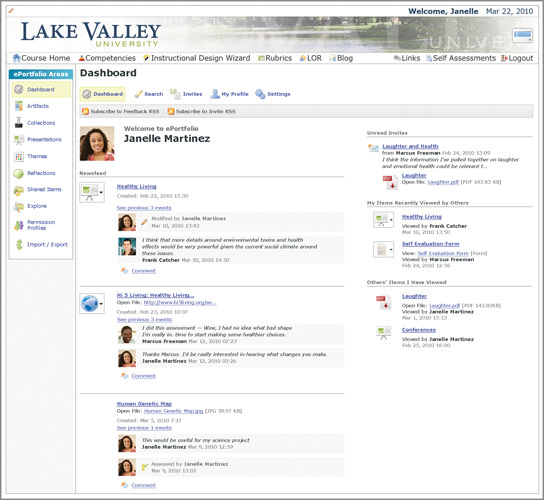
\includegraphics[width=0.8\textwidth]{CH4-F7-D2L}}
\caption[Desire2Learn ePortfolio example]{Desire2Learn ePortfolio example
\citep{Desire2LearnIncorporated2011}}
\label{fig:d2ep}
\end{figure}
 
\subsubsection{eFolio}

The Avenet Student eFolio\footnote{\url{http://www.avenetefolio.com}} is a
multimedia web site designed to store and attractively display resumes, academic
and career data and documentation, educational and career goals, achievements
and other meaningful information. Unlike a one-dimensional paper document, an
eFolio can "come alive" and provide a ``rich'' display, including documents,
images, audio, video, links, and detailed examples of accomplishments and
achievements.

\begin{figure}[htb]
\centering
\setlength\fboxsep{0pt}
\setlength\fboxrule{0.5pt}
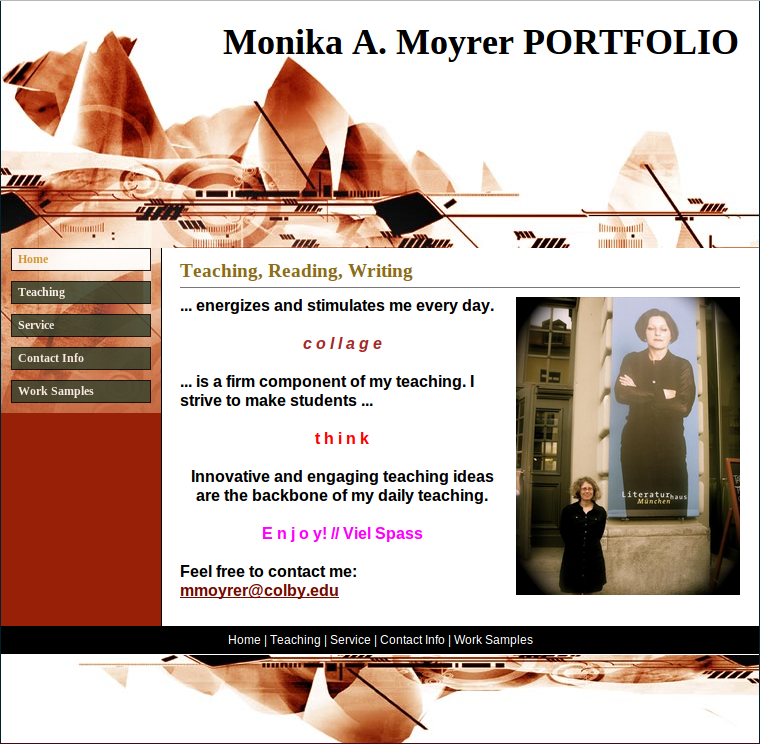
\includegraphics[width=0.8\textwidth]{CH4-F8-eFolio}
\caption[eFolio system example]{eFolio system example \citep{EFolioMinnesota2011}}
\label{fig:efolio}
\end{figure}

\section{Summary}

This review focuses on technical aspects of lifelong learning support.
Therefore, the following sections examine characteristics of the learning spaces
employed in universities and describe the issues related to the use of these
spaces in a universities environment. A review of \ep~systems is also
provided in these sections.

This review focuses on technical aspects of lifelong learning support.
Therefore, the following sections examine characteristics of the learning spaces
employed in universities and describe the issues related to the use of these
spaces in a universities environment. A review of \ep~systems is also
provided in these sections.

This review focuses on technical aspects of lifelong learning support.
Therefore, the following sections examine characteristics of the learning spaces
employed in universities and describe the issues related to the use of these
spaces in a universities environment. A review of \ep~systems is also
provided in these sections.